% !TeX spellcheck = en_US
\section{Project Specifications}

\textbf{AuctionHandler} is a distributed web-app in which users can sell their goods by creating Online Auctions. Registered users have the possibility to join an ongoing auction in order to buy a good in case they beat the concurrence by setting an higher offer on a given limited time.

\subsection{Use Cases}

An \textit{Unregistered User} can:
\begin{itemize}
	\item Register to the service
\end{itemize}
\noindent
A \textit{Unlogged User} can:
\begin{itemize}
	\item Login to the service
\end{itemize}
\noindent
A \textit{Logged User} can:
\begin{itemize}
	\item View the list of ongoing Auctions
	\item Create a new Auction
	\item Join an ongoing Auction
	\item Logout
	\item After Joining an Auction:
	\begin{itemize}
		\item Make an offer
		\item View list of participants
		\item View past offer history
		\item View the remaining time 
		\item Wait until the end of the Auction and then exit
		\item View Auction result
	\end{itemize}
\end{itemize}
The \textit{System} must:
\begin{itemize}
	\item Remember registered users
	\item Remember ongoing auctions
	\item Remember auction participants
	\item Choose in a unique way the auction winner
	\item Remember offers history
	\item Synchronize the remaining time, the auction participants, the offer history for an auction for each user
	\item Synchronize the list of ongoing auctions for each user
	
	
\end{itemize}
\begin{figure}[H]
	\centering
	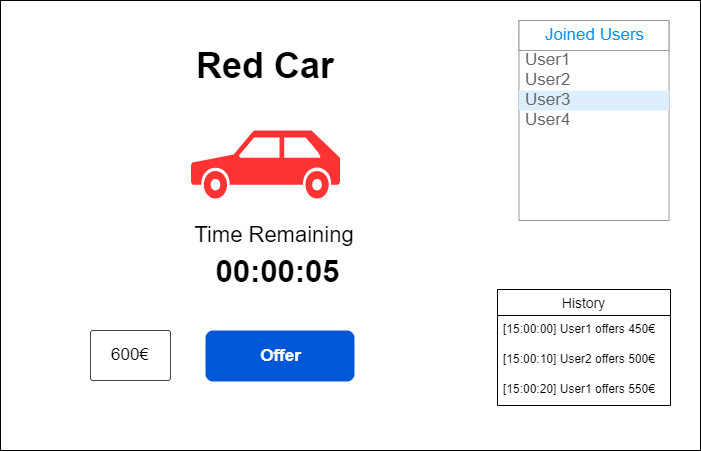
\includegraphics[width=0.7\linewidth]{img/wireframeDSMT.drawio}
	\caption{Mock-up of the main interface of the auction}
	\label{fig:wireframedsmt}
\end{figure}

\subsection{Synchronization and Communication Issues}\label{synchComIssues}
On the application we have the following synchronization and communication issues:
\begin{itemize}
	\item Client nodes need to be synchronized with the same remaining time of the auction, the same offer history for a given auction, the same list of joined users on a given auction and the same list of available ongoing auctions.
	\item In case a client makes a valid offer, the server will be in charge of  communicating to other clients nodes the information regarding the made offer. 
	\item In case a client creates a new auction, the server will be in charge of communicating to other clients the information regarding the newly created auction.
\end{itemize}
